% Template for Cogsci submission with R Markdown

% Stuff changed from original Markdown PLOS Template
\documentclass[10pt, letterpaper]{article}

\usepackage{cogsci}
\usepackage{pslatex}
\usepackage{float}
\usepackage{caption}

% amsmath package, useful for mathematical formulas
\usepackage{amsmath}

% amssymb package, useful for mathematical symbols
\usepackage{amssymb}

% hyperref package, useful for hyperlinks
\usepackage{hyperref}

% graphicx package, useful for including eps and pdf graphics
% include graphics with the command \includegraphics
\usepackage{graphicx}

% Sweave(-like)
\usepackage{fancyvrb}
\DefineVerbatimEnvironment{Sinput}{Verbatim}{fontshape=sl}
\DefineVerbatimEnvironment{Soutput}{Verbatim}{}
\DefineVerbatimEnvironment{Scode}{Verbatim}{fontshape=sl}
\newenvironment{Schunk}{}{}
\DefineVerbatimEnvironment{Code}{Verbatim}{}
\DefineVerbatimEnvironment{CodeInput}{Verbatim}{fontshape=sl}
\DefineVerbatimEnvironment{CodeOutput}{Verbatim}{}
\newenvironment{CodeChunk}{}{}

% cite package, to clean up citations in the main text. Do not remove.
\usepackage{apacite}

% KM added 1/4/18 to allow control of blind submission


\usepackage{color}

% Use doublespacing - comment out for single spacing
%\usepackage{setspace}
%\doublespacing


% % Text layout
% \topmargin 0.0cm
% \oddsidemargin 0.5cm
% \evensidemargin 0.5cm
% \textwidth 16cm
% \textheight 21cm

\title{Predicting ages of acquisition across 28 languages and dialects}


\author{{\large \bf Alvin W.M. Tan*, Georgia Loukatou*, Mika Braginsky} \\ Department of Psychology, Stanford University \AND {\large \bf Jessica Mankewitz} \\ Department of Psychology, University of Wisconsin--Madison \AND {\large \bf Michael C. Frank} \\ Department of Psychology, Stanford University}

\newlength{\cslhangindent}
\setlength{\cslhangindent}{1.5em}
\newenvironment{CSLReferences}%
  {}%
  {\par}

\begin{document}

\maketitle

\begin{abstract}
Research in early word learning has demonstrated that various factors
(e.g., word frequency) predict the ages of acquisition of different
words. However, a more comprehensive account requires the examination of
multiple levels of linguistic representation (e.g., phonological,
morphosyntactic, semantic) and language families (e.g., Indo-European,
Sino-Tibetan, Uralic). We studied 10 predictors of word ages of
acquisition across 28 languages and dialects, finding that words that
were more frequent, concrete, and associated with babies were learnt
earlier, whereas words that had greater length in phonemes and mean
length of utterance in words (MLU-w) were learnt later. There was no
reliable effect of other morphosyntactic predictors, or of phonological
neighbourhood size. We found evidence of a tradeoff between the
morphological complexity of a language and the effect of MLU-w for
predicates. Predictor coefficients revealed broad consistency across all
languages, along with variability that reflected language family
classifications.

\textbf{Keywords:}
Language acquisition; Word learning; Cross-linguistic; Age of
acquisition
\end{abstract}

\hypertarget{introduction}{%
\section{Introduction}\label{introduction}}

Why are some words learnt earlier than others? Despite the large
variation in the structure of different languages, children demonstrate
remarkably similar early lexical development across a wide swath of
languages, with highly overlapping first words (Frank, Braginsky,
Yurovsky, \& Marchman, 2021; Tardif et al., 2008), and similar emergence
of lexical categories (Caselli et al., 1995). The order of lexical
development can thus be used as a tool to understand the commonalities
and differences in the factors that predict word learning across
languages and lexical categories.

Such questions have led to a productive line of inquiry, with previous
research demonstrating that, in English, words learnt earlier tend to be
more frequent (Goodman, Dale, \& Li, 2008), be more iconic (Perry,
Perlman, \& Lupyan, 2015), and appear in shorter utterances (Swingley \&
Humphrey, 2018). The conclusions of these studies, however, were limited
in generalisability as they considered different sets of predictors, and
mostly focused only on English-learning children. In order to have a
more comprehensive understanding of early language learning, it is
important to capture two dimensions of variability: variability across
languages, and variability across levels of linguistic representation
(e.g., phonological, morphological, syntactic, and semantic). These
dimensions jointly provide information about how different sources of
information may be differentially relevant across languages of different
structures.

One study that has attempted to adopt this approach comes from
Braginsky, Yurovsky, Marchman, \& Frank (2019), who conducted a larger
scale cross-linguistic study across 10 languages, using a larger set of
predictors to determine their independent contributions to the
acquisition of different words (see also Frank et al., 2021). Overall,
they found strong consistent effects for predictors such as frequency
and concreteness, but little to no effect of predictors such as valence.

Nonetheless, there are two crucial limitations to their set of analyses.
First, among the predictors they considered, most were distributional
(frequency, frequency as sole word in utterance, frequency as last word
in utterance) or semantic (concreteness, babiness, valence, arousal),
with only one phonological predictor (length in phonemes) and one
syntactic predictor (mean length of utterance). Although there are
cross-linguistic and cultural differences in the distribution of words
in naturalistic speech, word frequencies are remarkably consistent,
especially for fundamental vocabulary (Calude \& Pagel, 2011), and
semantic representations also tend to exhibit similar organisations
cross-linguistically, at least within semantic domains (Lewis, Cahill,
Madnani, \& Evans, 2023). It is thus important to consider the full
range of levels of linguistic representation, particularly the levels
which are more likely to exhibit larger variation across languages,
viz.~morphological and syntactic factors.

The second limitation is that, of the 10 languages examined by Braginsky
et al. (2019), nine were Indo-European, and only one was not (Turkish).
As such, it is possible that some of the consistency that they observed
was in fact due to structural similarities among Indo-European
languages, as opposed to underlying patterns in language learning across
languages regardless of language family. To have a more accurate and
generalisable understanding of the factors driving early word learning,
it is imperative to study a more diverse set of languages, representing
a greater number of language families (see Kidd \& Garcia, 2022).

Hence, the present study aims to capture a more comprehensive view of
early word learning by including a broad set of predictors encompassing
phonological, morphological, syntactic, and semantic levels of
representation, as well as a large set of languages with particular
emphasis on non-Indo-European languages. We also examine the role of
lexical categories, given the theoretical predictions that different
lexical categories may be sensitive to different predictors. Together,
these directions will improve our characterisation of the consistency
and variation in early word learning across languages.

\hypertarget{method}{%
\section{Method}\label{method}}

\hypertarget{acquisition-data}{%
\subsection{Acquisition data}\label{acquisition-data}}

To study word learning in young children, we make use of data collected
via MacArthur--Bates Communicative Development Inventories (CDIs), which
are parent-report vocabulary checklists (Marchman, Dale, \& Fenson,
2023). CDIs are easy to administer and have been adapted into dozens of
different languages, with demonstrated reliability and validity as a
measure of language ability (Fenson et al., 2007; Mayor \& Plunkett,
2011), making them an effective method for capturing children's
vocabularies in many different contexts.

We used vocabulary data from Wordbank (Frank, Braginsky, Yurovsky, \&
Marchman, 2017), an open repository of CDI data contributed by various
researchers. These data included item-level data for each child, along
with associated demographic information such as the child's age. We
extracted productive vocabulary information from all forms, and
expressive vocabulary information from Words \& Gestures forms. Children
with language exposure to more than one language were excluded, and for
children with longitudinal data, only the first administration was used.
We included data from all languages for which all necessary resources
were available (see the Predictor data section for resources used),
amounting to 83934 children across 28 languages and dialects. An
overview of the data used is shown in Figure \ref{fig:descriptives}.

\begin{CodeChunk}
\begin{figure}[ht]

{\centering 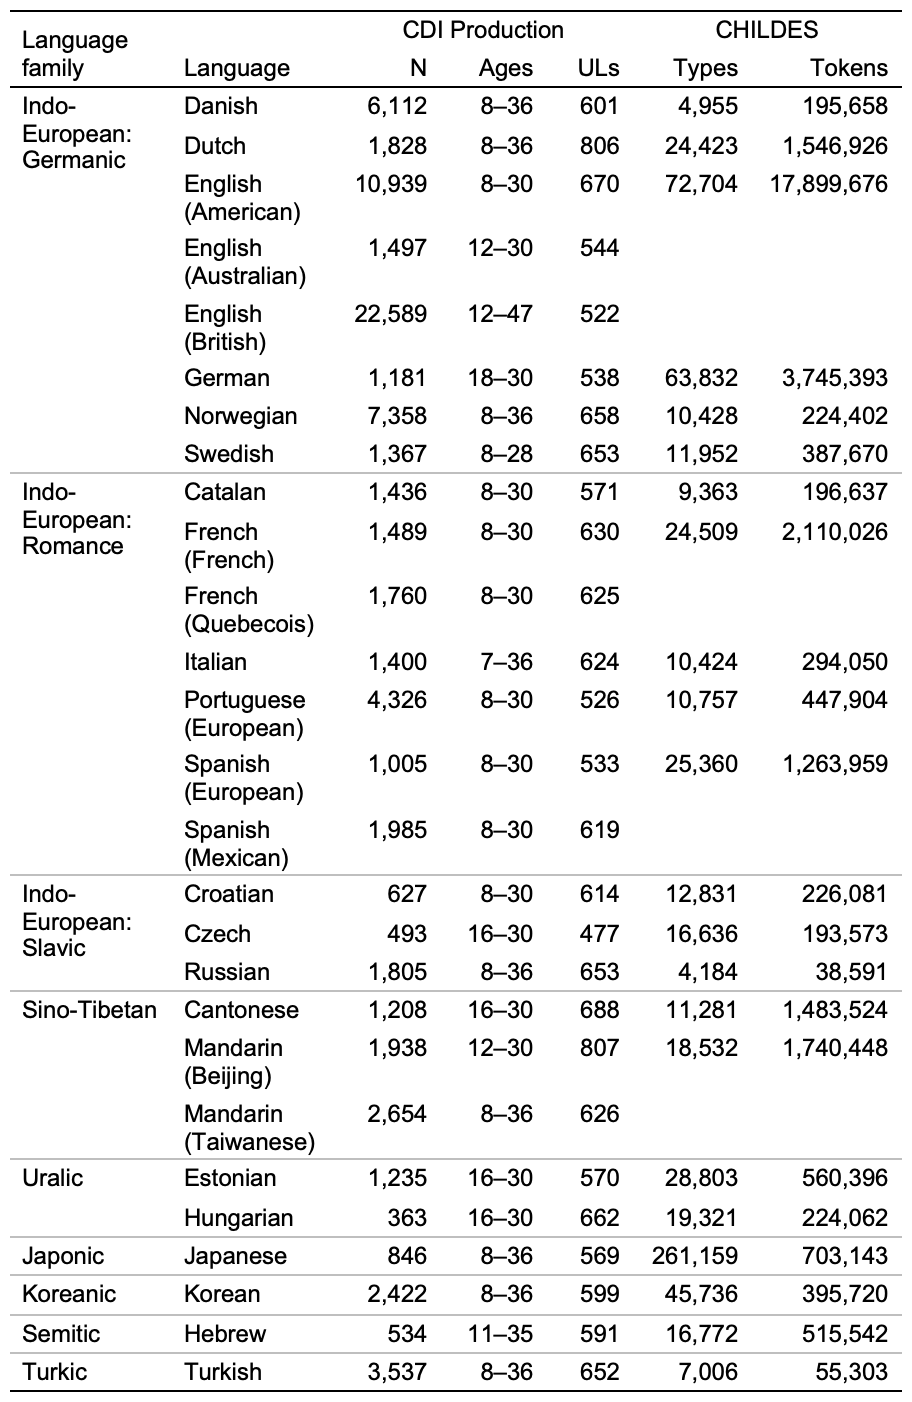
\includegraphics[width=240px]{figs/descriptives}

}

\caption[Descriptive statistics for data from Wordbank and CHILDES]{Descriptive statistics for data from Wordbank and CHILDES. N indicates number of children. ULs indicates number of unilemmas (see text).}\label{fig:descriptives}
\end{figure}
\end{CodeChunk}

In order to conduct comparisons across languages, we mapped items to
``universal lemmas'' or ``unilemmas'', which are approximate
cross-linguistic conceptual abstractions. For example, the items
``chat'' (FRA) and ``gato'' (SPA) map to the same unilemma, CAT. These
unilemmas were first constructed from glosses provided by the original
dataset contributors, then verified by native or proficient speakers of
the respective languages, and manually cleaned and consolidated to
improve overall consistency; more information about unilemma
construction can be found on Github {[}LINK REDACTED{]}. Note that some
items do not have corresponding unilemmas (e.g., language-specific items
that were not relevant cross-linguistically); these items were dropped
for analysis.

From these data, we derived ages of acquisition (AoAs) by fitting
Bayesian logistic regressions for each item, with word knowledge
(produces vs does not produce; understands vs does not understand) as
the outcome variable and age as the predictor variable. We used weakly
informative priors of \(\mathcal{N}(0, 2.5)\) for the intercept and
\(\mathcal{N}(0.3, 0.01)\) for the slopes. Then, the AoA is the age at
which 50\% of children are expected to know the word; this quantity can
be calculated as the negative of the intercept divided by the slope from
the fitted models (see Braginsky, Yurovsky, Marchman, \& Frank, 2016).

\hypertarget{predictors-of-age-of-acquisition}{%
\subsection{Predictors of age of
acquisition}\label{predictors-of-age-of-acquisition}}

For each language, we used corpora of child-directed speech from CHILDES
(MacWhinney, 2000) to calculate distributional information as well as
MLU-w.\footnote{Note that some of the languages (Hebrew and Russian) had
  CHILDES corpora that were transcribed in transliterated form instead
  of the original script; we used ad-hoc custom untransliteration
  scripts to enable matching to Wordbank, UniMorph, and UDPipe.} We also
used these corpora in conjunction with morphological segmentation
information from UniMorph (Batsuren, Bella, \& Giunchiglia, 2021;
Sylak-Glassman, 2016) and morphosyntactic parsing from UDPipe (Straka,
2018) to calculate morphosyntactic predictors. In addition, we used
previously collected adult psycholinguistic norms for the semantic
predictors (detailed below), and eSpeak NG (Vītoliņš, 2022) to obtain
phonological representations for the calculation of phonological
properties. An overview of the data and resources used for each item
property is shown in Figure \ref{fig:sources}.

\begin{CodeChunk}
\begin{figure}[ht]

{\centering 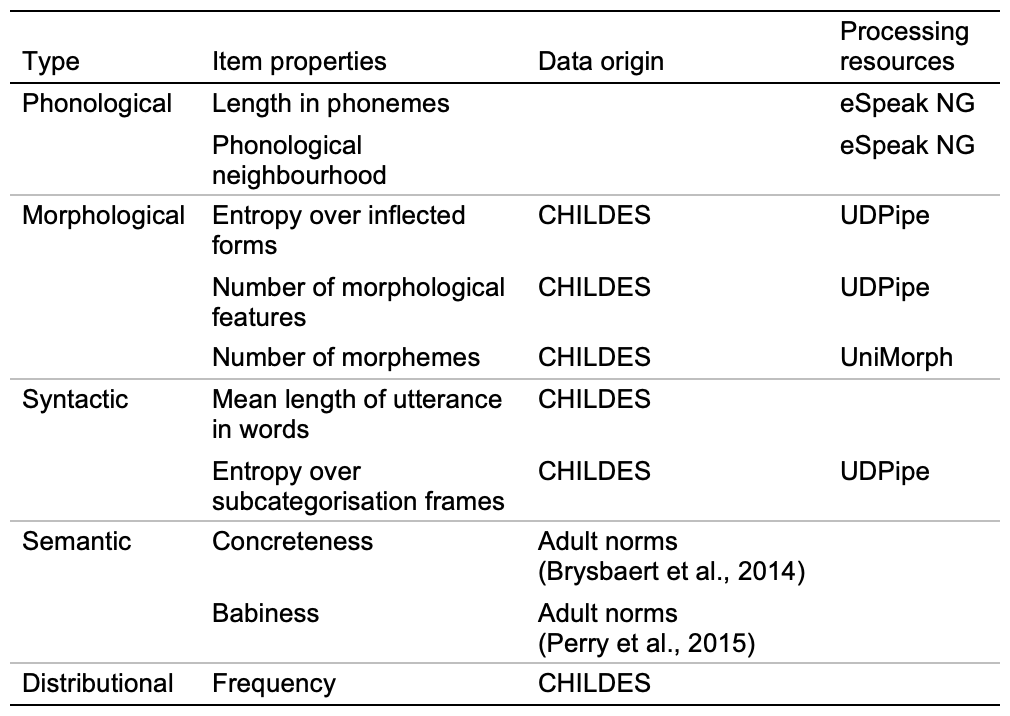
\includegraphics[width=240px]{figs/sources}

}

\caption[Item properties used, along with the data origins and resources used to derive item property values]{Item properties used, along with the data origins and resources used to derive item property values.}\label{fig:sources}
\end{figure}
\end{CodeChunk}

\textbf{Phonological properties.} For each item in each language, we
obtained all possible realisations of the item (e.g., ``cat'', ``cats'')
and generated phonological representations with eSpeak NG (Vītoliņš,
2022). These were directly used to calculate the mean length in
phonemes, as well as to measure the size of the phonological
neighbourhood, which was the number of other items that differed from
the target item by at most a Levenshtein distance of 2.

\textbf{Morphological properties.} To capture the morphological
properties of words, we considered both paradigmatic and syntagmatic
complexity. A paradigm refers to the set of related word forms of a
particular lemma (e.g., ``run'', ``runs'', ``running''), whereas a
syntagm refers to the set of words that can occur in sequence with a
particular lemma (e.g., ``the'', ``cat'', ``is'', ``running'').

We used two measures of morphological paradigmatic complexity, namely
entropy over inflected forms and number of morphological features, both
of which involved morphological parsing from UDPipe (Straka, 2018). For
each item, we found all tokens in CHILDES which had the same lemma as
the item, and calculated the Shannon entropy over the inflected forms
(Çöltekin \& Rama, 2023). The parsing also output morphological features
in the Universal Dependencies format (Nivre, Zeman, Ginter, \& Tyers,
2017), and we calculated the mean number of morphological features for
each item as an approximation of the size of the inflectional paradigm.

We also included one measure of morphological syntagmatic complexity,
namely mean number of morphemes; this made use of morphological
segmentation information from UniMorph (Batsuren et al., 2021;
Sylak-Glassman, 2016).

\textbf{Syntactic properties.} For each item, we calculated the MLU-w
for utterances in which the item appeared using CHILDES corpora, as a
proxy for the syntactic complexity of the item. We also used UDPipe to
parse the dependency structure of utterances, extracting the core and
oblique verbal dependents (objects, clausal complements, and obliques),
which served as a proxy for subcategorisation frames. We then calculated
the entropy over subcategorisation frames (Sharpe, Reddigari, Pylkkänen,
\& Marantz, 2019).

\textbf{Semantic properties.} We used previously collected adult norms
for concreteness (Brysbaert, Warriner, \& Kuperman, 2014) and babiness
(Perry et al., 2015) as our semantic predictors.

\textbf{Distributional properties.} We used CHILDES to calculate item
unigram frequencies, which were Laplace smoothed and log-transformed.

\textbf{Lexical categories.} Lexical categories were determined on the
basis of the conceptual categories presented on the CDIs (e.g.,
``Animals'', ``Action words'', ``Descriptive words''). We used the
categories ``nouns'' (for common nouns), ``predicates'' (for verbs,
adjectives, and adverbs), and ``function words'' (for closed class
words); all other items were classified as ``other''.

\hypertarget{predictor-processing}{%
\subsection{Predictor processing}\label{predictor-processing}}

\textbf{Residualisation.} Some of the item properties were a priori
correlated with one another. For example, shorter words tend to have
larger phonological neighbourhoods, and words with more morphological
features are likely to exhibit greater entropy over inflected forms. As
such, we conducted residualisation for phonological, morphological, and
syntactic properties. For each property type, we residualised the first
property (e.g, length in phonemes) out of all other properties (e.g.,
phonological neighbourhood), such that the coefficients of the other
properties would reflect their effects over and above any variance
explained by the first property.

\textbf{Imputation.} Some of the item properties contained missing data
depending on resource availability. We thus conducted iterative
imputation to fill in the missing values for each language by
iteratively imputing these values based on a linear regression fitting
that property from all other properties.

\textbf{Normalisation.} Finally, we centred and scaled all properties to
allow for direct comparison of standardised regression coefficients.

\textbf{Collinearity.} One possible concern for comparing coefficients
across languages is multicollinearity among predictor values. We
calculated variance inflation factors (VIFs) on models including all
predictors except for lexical categories (since models with interaction
effects are known to have inflated VIFs). The VIFs for each predictor in
each language was \(<3.5\), indicating low multicollinearity among
predictors.

\begin{CodeChunk}
\begin{figure*}[ht]

{\centering 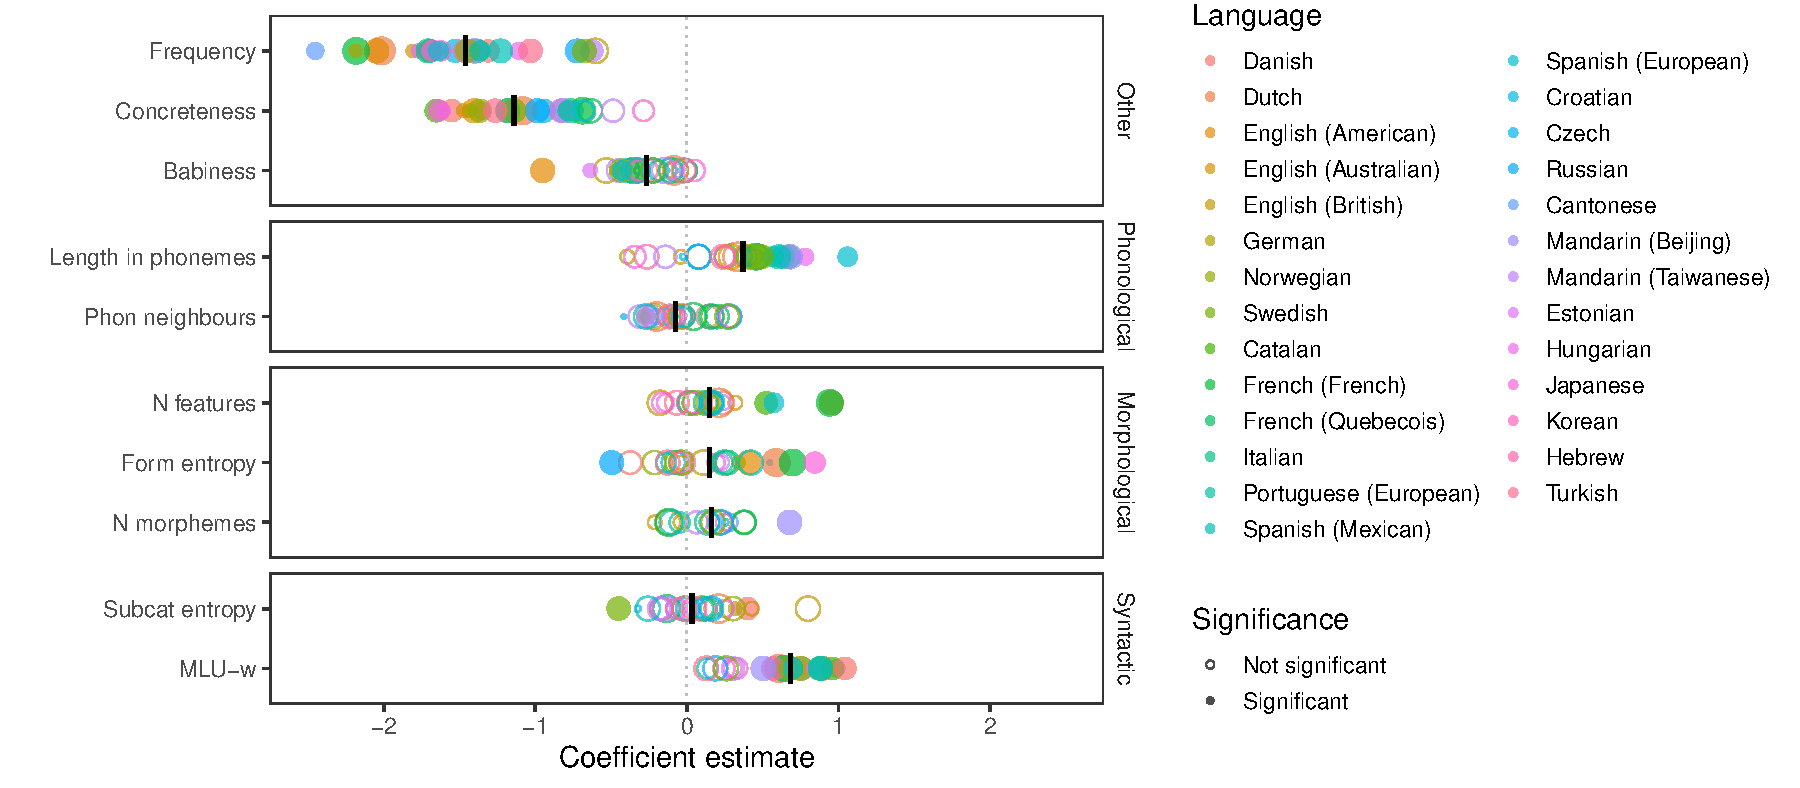
\includegraphics[width=500px]{figs/big_plot-1}

}

\caption[Maximum a posteriori estimates of coefficients predicting age of acquisition across all languages]{Maximum a posteriori estimates of coefficients predicting age of acquisition across all languages. Black vertical bars indicate estimate medians across all languages. Significance indicates whether the credible interval includes zero. Dot size indicates number of unilemmas.}\label{fig:big_plot}
\end{figure*}
\end{CodeChunk}

\hypertarget{analysis}{%
\subsection{Analysis}\label{analysis}}

We fit Bayesian linear models for each language, predicting the AoA of
each item from all item properties as well as their interactions with
the lexical category of the item. We used conservative informative
priors based on coefficient values from Braginsky et al. (2016), which
broadly fell in the range \((-2, 2)\); thus, we used a non-standardised
\(t\) distribution, \(t(3, 0, 2)\) as priors for coefficients. The
resultant standardised coefficients for each item property would reflect
its independent contribution to the AoA of the item, and interactions
with lexical categories would reflect how this contribution varies
across categories.

All code for data processing and analysis can be found on Github {[}LINK
REDACTED{]}.

\hypertarget{results}{%
\section{Results}\label{results}}

As a concise method to display model results, we plotted the maximum a
posteriori estimates for each predictor from the model fit on data from
each language. The main effects from all languages are shown in Figure
\ref{fig:big_plot}.

Model results demonstrated strong and consistent effects of frequency
(\(\bar{b}\) = -1.46), concreteness (\(\bar{b}\) = -1.14), and babiness
(\(\bar{b}\) = -0.27), as were previously found, such that words which
were more frequent, more concrete, and more associated with babies were
learnt earlier. For phonological predictors, longer words as measured in
phonemes were learnt later (\(\bar{b}\) = 0.37), but there was no
reliable effect of phonological neighbourhood size (\(\bar{b}\) = NA).
For morphological predictors, the number of morphological features
(\(\bar{b}\) = 0.15), entropy over inflected forms (\(\bar{b}\) = 0.15),
and number of morphemes (\(\bar{b}\) = 0.16) all did not have reliable
effects. For syntactic predictors, entropy over subcategorisation frames
did not have a reliable effect (\(\bar{b}\) = 0.03), while words that
had a greater MLU-w were learnt later (\(\bar{b}\) = 0.68).

\hypertarget{lexical-categories}{%
\subsection{Lexical categories}\label{lexical-categories}}

\begin{CodeChunk}
\begin{figure*}[ht]

{\centering 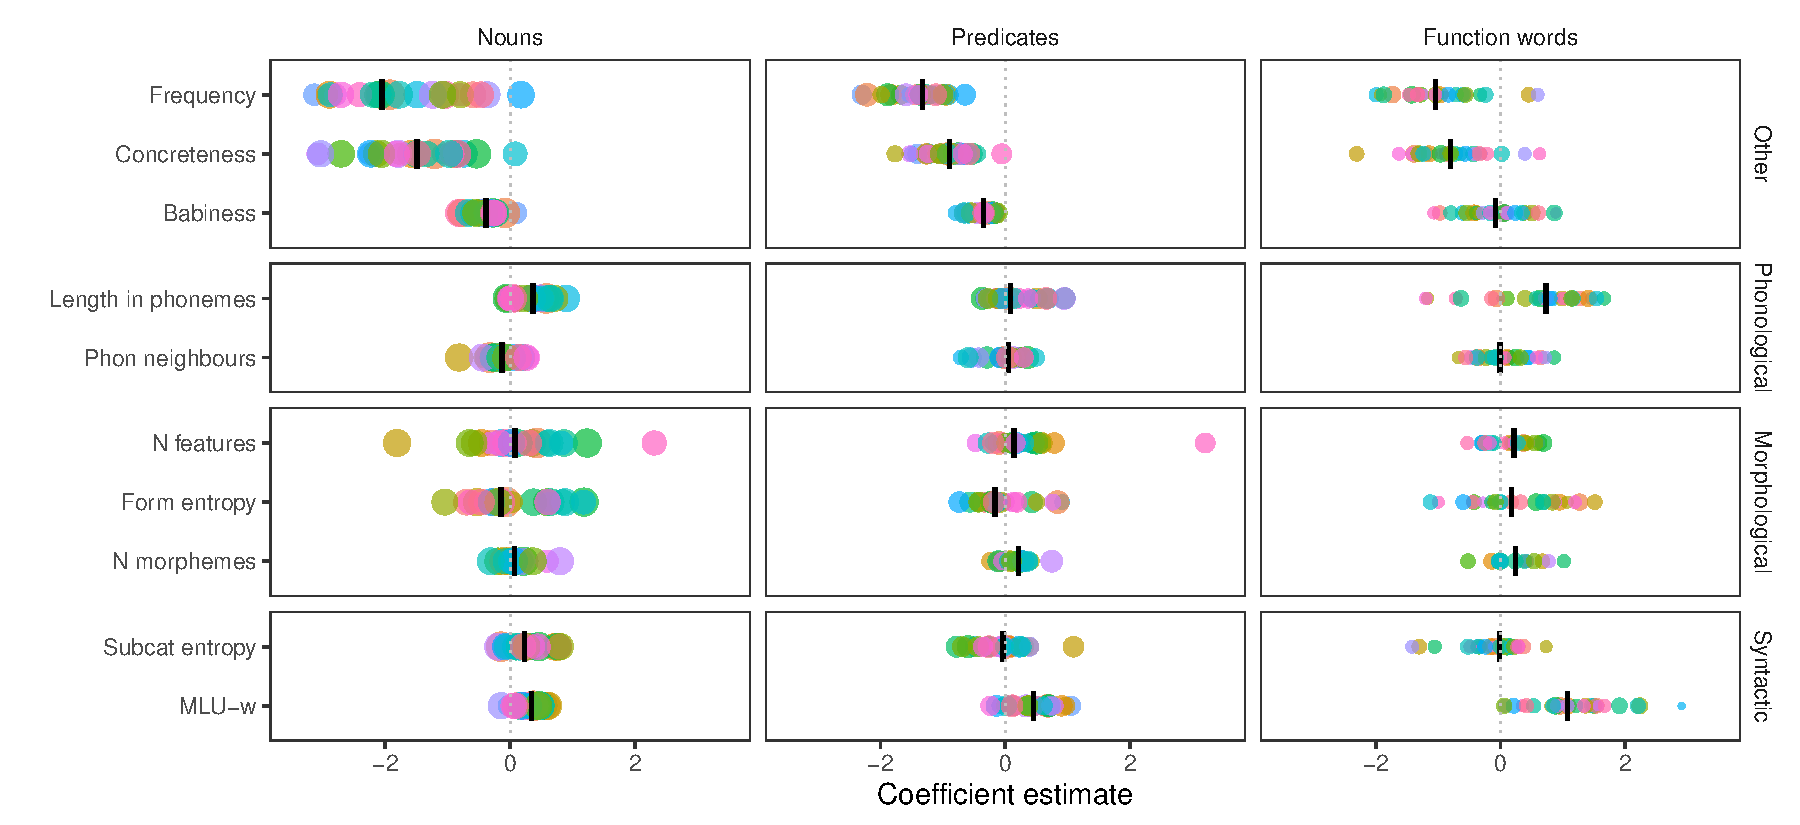
\includegraphics[width=500px]{figs/lc_plot-1}

}

\caption[Maximum a posteriori estimates of coefficients predicting age of acquisition across all languages, by lexical category]{Maximum a posteriori estimates of coefficients predicting age of acquisition across all languages, by lexical category. Black vertical bars indicate estimate medians across all languages. Dot size indicates number of unilemmas.}\label{fig:lc_plot}
\end{figure*}
\end{CodeChunk}

Estimates of predictor coefficients for different lexical categories are
shown in Figure \ref{fig:lc_plot}. Effects were mostly consistent across
lexical categories, with a few notable deviations. The effect of
babiness was attenuated for function words (\(\bar{b}\) = -0.01), and
the effect of length in phonemes was attenuated for predicates
(\(\bar{b}\) = 0.11). On the other hand, the effect of MLU-w was
enhanced for function words (\(\bar{b}\) = 0.43).

\hypertarget{correlations}{%
\subsection{Correlations}\label{correlations}}

\begin{CodeChunk}
\begin{figure}[ht]

{\centering 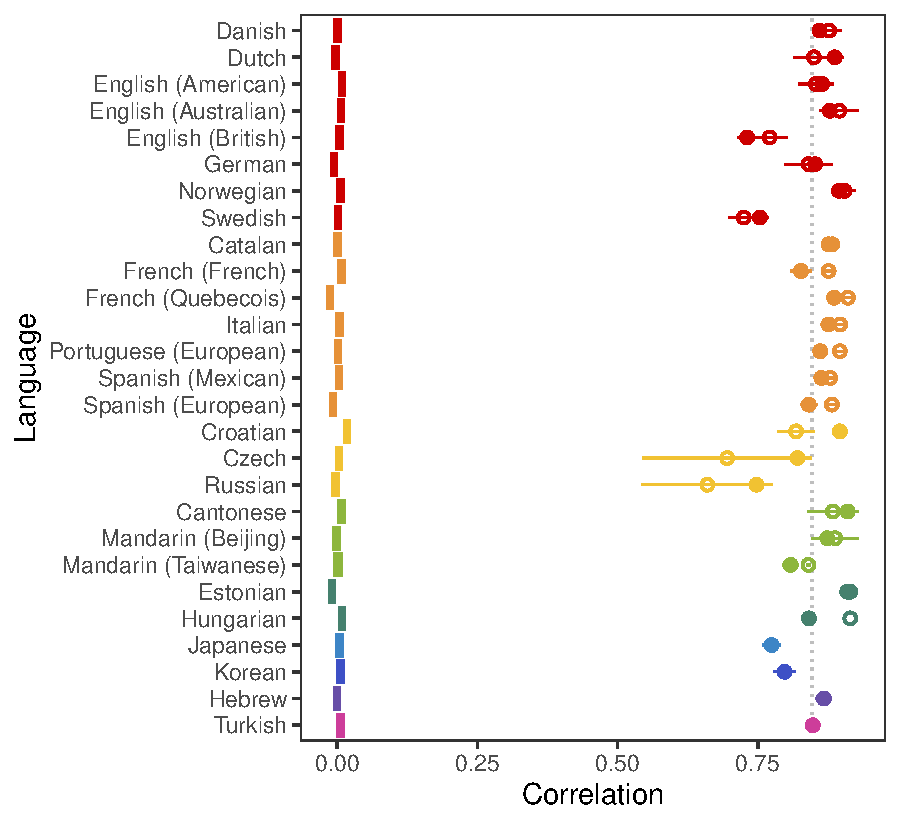
\includegraphics[width=240px]{figs/correlations-1}

}

\caption[Correlations of main effect coefficients across languages]{Correlations of main effect coefficients across languages. Filled circles indicate correlations with all other languages. Empty circles indicate correlations with other languages within the same language family. Shaded areas represent the bootstrapped randomised baseline. All ranges indicate 95\% confidence intervals. Dotted line indicates mean correlation. Colours represent language families.}\label{fig:correlations}
\end{figure}
\end{CodeChunk}

To understand the consistency and variability of predictors across
languages, we calculated the correlations between the coefficients of
the main effects for each language with all other languages, as well as
for other languages within its language family (for language families
with \(\ge 2\) included languages), as shown in Figure
\ref{fig:correlations}. The average correlation across languages was
relatively high (\(\bar{r}\) = 0.85), comparable to results found by
Braginsky et al.~(2019). Mean correlations within language families were
broadly numerically greater than those across language families,
indicating greater consistency within language families, except for
families in which particular languages had more idiosyncratic predictor
coefficients (English (British), Swedish, and Russian). We also
calculated a bootstrapped randomised baseline by permuting the predictor
labels for coefficients within each language and recalculating the
correlations with other languages; this procedure represented the
correlations that would be expected by chance. This baseline was
consistently close to 0, and was also consistently smaller than the
observed correlations.

\hypertarget{exploratory-analysis-morphological-complexity}{%
\subsection{Exploratory analysis: Morphological
complexity}\label{exploratory-analysis-morphological-complexity}}

As an exploratory analysis, we sought to understand the variation in the
effect sizes of the morphosyntactic predictors as a function of the
morphological complexity of the language, which may affect the
importance or informativeness of other morphosyntactic factors as cues
for word learning. Hence, for each combination of morphosyntactic factor
and lexical category, we conducted a linear regression with
morphosyntactic factor coefficient as the outcome variable and
morphological complexity as the predictor variable. We estimated
morphological complexity using the method from Bentz, Ruzsics, Koplenig,
\& Samardžic (2016), who used a composite index from 28 features of the
World Atlas of Linguistic Structures (Dryer \& Haspelmath, 2013),
ranging from 0 (least morphologically complex) to 1 (most
morphologically complex).

\begin{CodeChunk}
\begin{figure}[ht]

{\centering 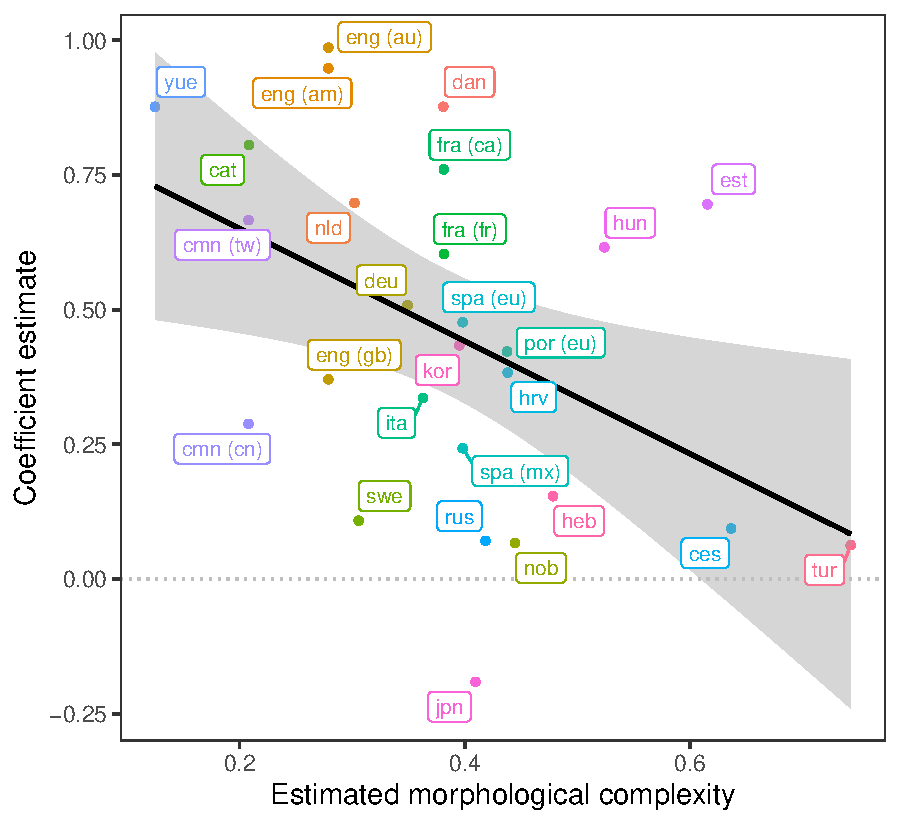
\includegraphics[width=240px]{figs/mlu_pred-1}

}

\caption[Coefficient of MLU-w for predicates against estimated morphological complexity]{Coefficient of MLU-w for predicates against estimated morphological complexity. Shaded area indicates standard error.}\label{fig:mlu_pred}
\end{figure}
\end{CodeChunk}

Only one model demonstrated a significant main effect of morphological
complexity, which was the model with MLU-w for predicates as the outcome
variable, as shown in Figure \ref{fig:mlu_pred}. The coefficient of the
effect of morphological complexity was negative (\(b\) = -1.05),
suggesting that languages with greater morphological complexity had a
smaller effect of MLU-w for the AoA of predicates.

\hypertarget{discussion}{%
\section{Discussion}\label{discussion}}

By examining the predictors of AoA across different languages, we found
that words with higher frequency, concreteness, and babiness were learnt
earlier, whereas words with greater length in phonemes and MLU-w were
learnt later. We found that these effects were generally consistent
across typologically diverse languages, suggesting that early word
learning broadly taps on similar sources of linguistic information
despite disparities in the realisations of such information across
languages. These effects also concur with those found by previous work
(Braginsky et al., 2016, 2019).

In contrast, there was little evidence overall of any effect of
morphosyntactic predictors. This finding is surprising, given the
diversity in morphosyntax across the languages included in our study.
One possible explanation for the lack of a reliable effect is the
operationalisation of our metrics. When completing the CDI, caregivers
may indicate that their child is able to say a word even if the specific
produced form is reduced or otherwise idiosyncratic, and thus the child
need not have a complete grasp of the inflectional paradigm of the word.
As such, we adopted metrics that were appropriate at the lemma level
(e.g., information about the complexity of lemma paradigms).
Morphosyntactic predictors may be more crucial when learning other
aspects of morphosyntax, particularly at the form level (e.g., deploying
appropriately inflected forms).

We also did not find an effect of phonological neighbourhood size, which
contrasts with previous work suggesting that words with larger
phonological neighbourhoods were more likely to be learnt (Fourtassi,
Bian, \& Frank, 2020; Jones \& Brandt, 2019). In particular, Fourtassi
et al. (2020) used a relatively similar method of calculation to the
present study (considering only CDI words as potential neighbours and
controlling for frequency), but still found an effect of phonological
neighbourhood. The difference in results may be due to the fact that
they restricted their analyses to CDI nouns, whereas we also included
predicates and function words in our reference corpora. Further research
is necessary to determine whether lexical category-specific phonological
networks may be more relevant for early word learning.

Our results also demonstrated broad consistency across lexical
categories, with some variation for particular predictors. This
variation supports the hypothesis that words from different lexical
categories may be learnt in different ways, such that different word
properties may contribute to differing extents. For example, semantic
factors (such as babiness) may be less important for function words,
whereas syntactic complexity (as measured by MLU-w) may be more
important, and word length may not be the bottleneck for acquiring
predicates. These results align with the predictions made by other
theories of early language acquisition. Notably, syntactic bootstrapping
theory (Gleitman, 1990) suggests that syntactic information may be more
crucial for acquiring the meanings of function words, while
comparatively, noun semantics can be learnt more easily from direct
cross-situational mapping (Monaghan, Mattock, Davies, \& Smith, 2015).

Indeed, the differing roles of various predictors across lexical
categories is also demonstrated by the relationship between
morphological complexity and the effect of MLU-w, specifically for
predicates (but not nouns or function words). This finding provides some
support for the competition model (Bates \& Macwhinney, 1982), which
suggests that differential cue availability and reliability across
languages may lead to differences in the AoA of different linguistic
structures. For languages with greater morphological complexity, the
reliability of morphological markers may lead to a lessened effect of
syntactic complexity, and vice versa, suggesting a trade-off between the
two dimensions of complexity (see Bentz, Gutierrez-Vasques, Sozinova, \&
Samardžić, 2022; but cf. Benítez-Burraco, Chen, \& Gil, 2024). It is
important to emphasise that this analysis is exploratory in nature, and
the results should be interpreted with caution, especially because of
the small number of data points.

The current study represents an attempt to understand the process of
word learning across a large range of languages, so as to better
characterise the role of linguistic diversity in early language
learning. In particular, we expanded the range of languages under
consideration, using data from 28 languages and varieties, of which 10
(i.e., more than a third) were non-Indo-European. Nonetheless, there
remained an Indo-European bias, and certain language families were also
underrepresented, especially language families across Africa and
Oceania. Much more research in those languages is necessary for a truly
comprehensive view of early word learning, as encouraged by Kidd \&
Garcia (2022) and others.

Additionally, even for the languages which were included in our study,
there was variation in the amount and quality of coverage for the
different resources used. For example, some languages have more UniMorph
data on verbs than other lexical categories, which may have resulted in
biassed predictor values. The consistency in observed predictor values
suggests that such a potential bias was not very large in magnitude, but
it remains crucial to increase resource availability in understudied
languages to permit more accurate study of these languages.

Nonetheless, the current work presents a case for the use of a diverse
range of language samples to study the consistency and variability of
early language learning across languages and across levels of
representation. Additionally, it is worth highlighting that this
research was only made possible through the availability of multiple
open data and open science resources, emphasising the importance of open
science practices. Continued advancements in data collection and sharing
from a greater breadth of languages will certainly help to further our
understanding of language acquisition in young children.

\hypertarget{references}{%
\section{References}\label{references}}

\setlength{\parindent}{-0.1in}
\setlength{\leftskip}{0.125in}

\noindent

\hypertarget{refs}{}
\begin{CSLReferences}
\leavevmode\vadjust pre{\hypertarget{ref-batesFunctionalistApproachesGrammar1982}{}}%
Bates, E., \& Macwhinney, B. (1982). Functionalist approaches to
grammar. In E. Wanner \& L. R. Gleitman (Eds.), \emph{Child {Language}:
{The State} of the {Art}}. {Cambridge}: {Cambridge University Press}.

\leavevmode\vadjust pre{\hypertarget{ref-batsurenMorphyNetLargeMultilingual2021}{}}%
Batsuren, K., Bella, G., \& Giunchiglia, F. (2021). {MorphyNet}: A
{Large Multilingual Database} of {Derivational} and {Inflectional
Morphology}. In \emph{Proceedings of the 18th {SIGMORPHON Workshop} on
{Computational Research} in {Phonetics}, {Phonology}, and {Morphology}}
(pp. 39--48). {Online}: {Association for Computational Linguistics}.
http://doi.org/\href{https://doi.org/10.18653/v1/2021.sigmorphon-1.5}{10.18653/v1/2021.sigmorphon-1.5}

\leavevmode\vadjust pre{\hypertarget{ref-benitez-burracoAbsenceTradeoffMorphological2024}{}}%
Benítez-Burraco, A., Chen, S., \& Gil, D. (2024). The absence of a
trade-off between morphological and syntactic complexity.
\emph{Frontiers in Language Sciences}, \emph{3}. Retrieved from
\url{https://www.frontiersin.org/articles/10.3389/flang.2024.1340493}

\leavevmode\vadjust pre{\hypertarget{ref-bentzComplexityTradeoffsEquicomplexity2022}{}}%
Bentz, C., Gutierrez-Vasques, X., Sozinova, O., \& Samardžić, T. (2022).
Complexity trade-offs and equi-complexity in natural languages: A
meta-analysis. \emph{Linguistics Vanguard}.
http://doi.org/\href{https://doi.org/10.1515/lingvan-2021-0054}{10.1515/lingvan-2021-0054}

\leavevmode\vadjust pre{\hypertarget{ref-bentzComparisonMorphologicalComplexity2016}{}}%
Bentz, C., Ruzsics, T., Koplenig, A., \& Samardžic, T. (2016). A
{Comparison Between Morphological Complexity Measures}: {Typological
Data} vs. {Language Corpora}. In \emph{Proceedings of the {Workshop} on
{Computational Linguistics} for {Linguistic Complexity}}. {Osaka,
Japan}.

\leavevmode\vadjust pre{\hypertarget{ref-braginskyUhohTomorrowPredicting2016}{}}%
Braginsky, M., Yurovsky, D., Marchman, V. A., \& Frank, M. C. (2016).
From uh-oh to tomorrow {Predicting} age of acquisition for early words
across languages. In \emph{Proceedings of the 38th {Annual Meeting} of
the {Cognitive Science Society}} (pp. 1691--1696). {Philadelphia, PA}.

\leavevmode\vadjust pre{\hypertarget{ref-braginskyConsistencyVariabilityChildren2019}{}}%
Braginsky, M., Yurovsky, D., Marchman, V. A., \& Frank, M. C. (2019).
Consistency and {Variability} in {Children}'s {Word Learning Across
Languages}. \emph{Open Mind: Discoveries in Cognitive Science},
\emph{3}, 52--67.
http://doi.org/\href{https://doi.org/10.1162/opmi_a_00026}{10.1162/opmi\_a\_00026}

\leavevmode\vadjust pre{\hypertarget{ref-brysbaertConcretenessRatings402014}{}}%
Brysbaert, M., Warriner, A. B., \& Kuperman, V. (2014). Concreteness
ratings for 40 thousand generally known {English} word lemmas.
\emph{Behavior Research Methods}, \emph{46}(3), 904--911.
http://doi.org/\href{https://doi.org/10.3758/s13428-013-0403-5}{10.3758/s13428-013-0403-5}

\leavevmode\vadjust pre{\hypertarget{ref-caludeHowWeUse2011}{}}%
Calude, A. S., \& Pagel, M. (2011). How do we use language? {Shared}
patterns in the frequency of word use across 17 world languages.
\emph{Philosophical Transactions of the Royal Society B: Biological
Sciences}, \emph{366}(1567), 1101--1107.
http://doi.org/\href{https://doi.org/10.1098/rstb.2010.0315}{10.1098/rstb.2010.0315}

\leavevmode\vadjust pre{\hypertarget{ref-caselliCrosslinguisticStudyEarly1995}{}}%
Caselli, M. C., Bates, E., Casadio, P., Fenson, J., Fenson, L., Sanderl,
L., \& Weir, J. (1995). A cross-linguistic study of early lexical
development. \emph{Cognitive Development}, \emph{10}(2), 159--199.
http://doi.org/\href{https://doi.org/10.1016/0885-2014(95)90008-X}{10.1016/0885-2014(95)90008-X}

\leavevmode\vadjust pre{\hypertarget{ref-coltekinWhatComplexityMeasures2023}{}}%
Çöltekin, Ç., \& Rama, T. (2023). What do complexity measures measure?
{Correlating} and validating corpus-based measures of morphological
complexity. \emph{Linguistics Vanguard}, \emph{9}(s1), 27--43.
http://doi.org/\href{https://doi.org/10.1515/lingvan-2021-0007}{10.1515/lingvan-2021-0007}

\leavevmode\vadjust pre{\hypertarget{ref-dryerWorldAtlasLanguage2013}{}}%
Dryer, M. S., \& Haspelmath, M. (Eds.). (2013). \emph{The {World Atlas}
of {Language Structures}}. Data set, {Zenodo}.
http://doi.org/\href{https://doi.org/10.5281/zenodo.7385533}{10.5281/zenodo.7385533}

\leavevmode\vadjust pre{\hypertarget{ref-fensonMacArthurBatesCommunicativeDevelopment2007}{}}%
Fenson, L., Marchman, V. A., Thal, D. J., Dale, P. S., Reznick, J. S.,
\& Bates, E. (2007). \emph{{MacArthur-Bates Communicative Development
Inventories}: {User}'s {Guide} and {Technical Manual}}. {Paul H. Brookes
Publishing Company}.

\leavevmode\vadjust pre{\hypertarget{ref-fourtassiGrowthChildrenSemantic2020}{}}%
Fourtassi, A., Bian, Y., \& Frank, M. C. (2020). The {Growth} of
{Children}'s {Semantic} and {Phonological Networks}: {Insight From} 10
{Languages}. \emph{Cognitive Science}, \emph{44}(7), e12847.
http://doi.org/\href{https://doi.org/10.1111/cogs.12847}{10.1111/cogs.12847}

\leavevmode\vadjust pre{\hypertarget{ref-frankWordbankOpenRepository2017}{}}%
Frank, M. C., Braginsky, M., Yurovsky, D., \& Marchman, V. A. (2017).
Wordbank: An open repository for developmental vocabulary data.
\emph{Journal of Child Language}, \emph{44}(3), 677--694.
http://doi.org/\href{https://doi.org/10.1017/S0305000916000209}{10.1017/S0305000916000209}

\leavevmode\vadjust pre{\hypertarget{ref-frankVariabilityConsistencyEarly2021}{}}%
Frank, M. C., Braginsky, M., Yurovsky, D., \& Marchman, V. A. (2021).
\emph{Variability and {Consistency} in {Early Language Learning}: {The
Wordbank Project}}. {Cambridge, MA, USA}: {MIT Press}.

\leavevmode\vadjust pre{\hypertarget{ref-gleitmanStructuralSourcesVerb1990}{}}%
Gleitman, L. (1990). The {Structural Sources} of {Verb Meanings}.
\emph{Language Acquisition}, \emph{1}(1), 3--55. Retrieved from
\url{https://www.jstor.org/stable/20011341}

\leavevmode\vadjust pre{\hypertarget{ref-goodmanDoesFrequencyCount2008}{}}%
Goodman, J. C., Dale, P. S., \& Li, P. (2008). Does frequency count?
{Parental} input and the acquisition of vocabulary. \emph{Journal of
Child Language}, \emph{35}(3), 515--531.
http://doi.org/\href{https://doi.org/10.1017/S0305000907008641}{10.1017/S0305000907008641}

\leavevmode\vadjust pre{\hypertarget{ref-jonesChildrenReallyAcquire2019}{}}%
Jones, S. D., \& Brandt, S. (2019). Do children really acquire dense
neighbourhoods? \emph{Journal of Child Language}, \emph{46}(6),
1260--1273.
http://doi.org/\href{https://doi.org/10.1017/S0305000919000473}{10.1017/S0305000919000473}

\leavevmode\vadjust pre{\hypertarget{ref-kiddHowDiverseChild2022}{}}%
Kidd, E., \& Garcia, R. (2022). How diverse is child language
acquisition research? \emph{First Language}, \emph{42}(6), 703--735.
http://doi.org/\href{https://doi.org/10.1177/01427237211066405}{10.1177/01427237211066405}

\leavevmode\vadjust pre{\hypertarget{ref-lewisLocalSimilarityGlobal2023}{}}%
Lewis, M., Cahill, A., Madnani, N., \& Evans, J. (2023). Local
similarity and global variability characterize the semantic space of
human languages. \emph{Proceedings of the National Academy of Sciences},
\emph{120}(51), e2300986120.
http://doi.org/\href{https://doi.org/10.1073/pnas.2300986120}{10.1073/pnas.2300986120}

\leavevmode\vadjust pre{\hypertarget{ref-macwhinneyCHILDESProjectTools2000}{}}%
MacWhinney, B. (2000). \emph{The {CHILDES Project}: {Tools} for
analyzing talk.} (3rd ed.). {Mahwah, NJ}: {Lawrence Erlbaum Associates}.

\leavevmode\vadjust pre{\hypertarget{ref-marchmanMacArthurBatesCommunicativeDevelopment2023}{}}%
Marchman, V. A., Dale, P., \& Fenson, L. (2023). \emph{{MacArthur-Bates
Communicative Development Inventories User}'s {Guide} and {Technical
Manual}} (3rd edition). {Brookes Publishing Co.}

\leavevmode\vadjust pre{\hypertarget{ref-mayorStatisticalEstimateInfant2011}{}}%
Mayor, J., \& Plunkett, K. (2011). A statistical estimate of infant and
toddler vocabulary size from {CDI} analysis. \emph{Developmental
Science}, \emph{14}(4), 769--785.
http://doi.org/\href{https://doi.org/10.1111/j.1467-7687.2010.01024.x}{10.1111/j.1467-7687.2010.01024.x}

\leavevmode\vadjust pre{\hypertarget{ref-monaghanGavagaiGavagaiDoes2015}{}}%
Monaghan, P., Mattock, K., Davies, R. A. I., \& Smith, A. C. (2015).
Gavagai {Is} as {Gavagai Does}: {Learning Nouns} and {Verbs From
Cross-Situational Statistics}. \emph{Cognitive Science}, \emph{39}(5),
1099--1112.
http://doi.org/\href{https://doi.org/10.1111/cogs.12186}{10.1111/cogs.12186}

\leavevmode\vadjust pre{\hypertarget{ref-nivreUniversalDependencies2017}{}}%
Nivre, J., Zeman, D., Ginter, F., \& Tyers, F. (2017). Universal
{Dependencies}. In A. Klementiev \& L. Specia (Eds.), \emph{Proceedings
of the 15th {Conference} of the {European Chapter} of the {Association}
for {Computational Linguistics}: {Tutorial Abstracts}}. {Valencia,
Spain}: {Association for Computational Linguistics}. Retrieved from
\url{https://aclanthology.org/E17-5001}

\leavevmode\vadjust pre{\hypertarget{ref-perryIconicityEnglishSpanish2015}{}}%
Perry, L. K., Perlman, M., \& Lupyan, G. (2015). Iconicity in {English}
and {Spanish} and {Its Relation} to {Lexical Category} and {Age} of
{Acquisition}. \emph{PLoS ONE}, \emph{10}(9), e0137147.
http://doi.org/\href{https://doi.org/10.1371/journal.pone.0137147}{10.1371/journal.pone.0137147}

\leavevmode\vadjust pre{\hypertarget{ref-sharpeAutomaticAccessVerb2019}{}}%
Sharpe, V., Reddigari, S., Pylkkänen, L., \& Marantz, A. (2019).
Automatic access to verb continuations on the lexical and categorical
levels: Evidence from {MEG}. \emph{Language, Cognition and
Neuroscience}, \emph{34}(2), 137--150.
http://doi.org/\href{https://doi.org/10.1080/23273798.2018.1531139}{10.1080/23273798.2018.1531139}

\leavevmode\vadjust pre{\hypertarget{ref-strakaUDPipePrototypeCoNLL2018}{}}%
Straka, M. (2018). {UDPipe} 2.0 {Prototype} at {CoNLL} 2018 {UD Shared
Task}. In D. Zeman \& J. Hajič (Eds.), \emph{Proceedings of the {CoNLL}
2018 {Shared Task}: {Multilingual Parsing} from {Raw Text} to {Universal
Dependencies}} (pp. 197--207). {Brussels, Belgium}: {Association for
Computational Linguistics}.
http://doi.org/\href{https://doi.org/10.18653/v1/K18-2020}{10.18653/v1/K18-2020}

\leavevmode\vadjust pre{\hypertarget{ref-swingleyQuantitativeLinguisticPredictors2018}{}}%
Swingley, D., \& Humphrey, C. (2018). Quantitative {Linguistic
Predictors} of {Infants}' {Learning} of {Specific English Words}.
\emph{Child Development}, \emph{89}(4), 1247--1267.
http://doi.org/\href{https://doi.org/10.1111/cdev.12731}{10.1111/cdev.12731}

\leavevmode\vadjust pre{\hypertarget{ref-sylak-glassmanCompositionUseUniversal2016}{}}%
Sylak-Glassman, J. (2016, June 2). The {Composition} and {Use} of the
{Universal Morphological Feature Schema} ({UniMorph Schema}). Retrieved
from \url{https://unimorph.github.io/doc/unimorph-schema.pdf}

\leavevmode\vadjust pre{\hypertarget{ref-tardifBabyFirst102008}{}}%
Tardif, T., Fletcher, P., Liang, W., Zhang, Z., Kaciroti, N., \&
Marchman, V. A. (2008). Baby's first 10 words. \emph{Developmental
Psychology}, \emph{44}(4), 929--938.
http://doi.org/\href{https://doi.org/10.1037/0012-1649.44.4.929}{10.1037/0012-1649.44.4.929}

\leavevmode\vadjust pre{\hypertarget{ref-vitolinsESpeakNG2022}{}}%
Vītoliņš, V. (2022). {eSpeak NG} (Version 1.51). Retrieved from
\url{https://github.com/espeak-ng/espeak-ng}

\end{CSLReferences}

\bibliographystyle{apacite}


\end{document}
